\section{Úvodní pojmy}
\label{sec:uvodni-pojmy}

Žádná matematická disciplína se neobejde bez pochopení základů logiky a teorie
množin. Pro jistotu zde nejnutnější části připomeneme, ale tyto krátké úryvky
nezamýšlejí naučit, leč osvěžit.

\subsection{Logické spojky a kvantifikátory}
\label{ssec:logicke-spojky-a-kvantifikatory}

\begin{definition}[Výrok]
 Výrokem nazveme jakoukoli větu, o které lze rozhodnout, zda je pravdivá, či
 nikoliv.
\end{definition}

\begin{example}
 Věty \uv{Je mi zle.} a \uv{Sumec je drůbež.} jsou výroky, zatímco \uv{Tvoje
 máma.} a \uv{Cos' dostala z matiky?} nikoliževěk.

 Je též dlužno mít na paměti, že naše znalost pravdivosti věty nemění nic na
 tom, jestli daná věta je, nebo není výrokem. Třeba \uv{Do pěti století
 kolonizujeme celou Sluneční soustavu.} je zcela jistě výrok.
\end{example}

Další text vyžaduje znalost operátorů $\neg, \wedge, \vee, \Rightarrow$ a
$\Leftrightarrow$. Je-li $x$ výrok \uv{Prší.} a $y$ výrok \uv{Vezmu si
deštník.}, pak
\begin{itemize}
 \item výrok $\neg x$ znamená \uv{\textbf{Ne}prší.},
 \item výrok $x \wedge y$ znamená \uv{Prší \textbf{a} vezmu si deštník.},
 \item výrok $x \vee y$ znamená \uv{Prší \textbf{nebo} si vezmu deštník.},
 \item výrok $x \Rightarrow y$ znamená \uv{\textbf{Když} prší, \textbf{tak} si
  vezmu deštník.} a
 \item výrok $x \Leftrightarrow y$ znamená \uv{Prší, \textbf{právě tehdy když}
  si vezmu deštník.}
\end{itemize}

\begin{warning}\hfill
 \vspace*{-\parskip}
 \begin{itemize}
  \item Logická spojka $ \vee $ \textbf{není výlučná}. Tedy $x \vee y$ platí
   v situaci, kdy
   \begin{itemize}
    \item platí pouze $x$,
    \item platí pouze $y$,
    \item platí $x$ i $y$.
   \end{itemize}
  \item Výrok $x \Rightarrow y$ je vždy \textbf{pravdivý}, pokud $x$ je
   \textbf{lživý}. Jinak řečeno, $x \Rightarrow y$ platí za situace, kdy
   \begin{itemize}
    \item platí $x$ i $y$,
    \item neplatí $x$ a platí $y$,
    \item neplatí $x$ a neplatí $y$.
   \end{itemize}
 \end{itemize}
\end{warning}

Jako znalost logických spojek je kritická i znalost kvantifikátorů $ \forall $ 
a $ \exists $, které se čtou \uv{pro všechny} a \uv{existuje}, resp.

Pokud je $p(x)$ výrok závislý na proměnné $x$ (třeba \uv{$x$ je sudé.}), pak
výrok
\begin{itemize}
 \item $ \forall x \in \N: p(x)$ zní \uv{Všechna přirozená čísla jsou sudá.} a
 \item $ \exists x \in \N: p(x)$ zní \uv{Existuje sudé přirozené číslo.}
\end{itemize}
Budeme rovněž užívat kvantifikátory $ \exists!$ a $\nexists$, které znamenají
\uv{existuje přesně jeden} a \uv{neexistuje}.

Podáno intutivně: chci-li tvrdit, že $ \forall x \in \N:p(x)$, musím dokázat,
že ať mi nepřítel dá \textbf{jakéḱoliv} přirozené číslo $x$, tak $p(x)$ platí.
Naopak, dokázat $ \exists x \in \N: p(x)$ je obvykle zásadně jednodušší, neboť
musím pouze najít \textbf{jedno} přirozené číslo $x$, pro které $p(x)$ platí.

\subsection{Množiny}
\label{ssec:mnoziny}

Požaduji znalost značek $ \in,  \cap,  \cup ,  \setminus ,  \times $ a $
\subseteq $. Pro připomenutí, jsou-li $A,B$ dvě množiny, pak
\begin{itemize}
 \item výrok $x \in A$ říká, že \uv{$x$ je prvkem $A$.} nebo \uv{ $x$ patří do
  $A$.};
 \item  $A \cap B$ je \textbf{průnik} $A$ s $B$, čili množina obsahující
  prvky, které patří jak do $A$, tak do $B$;
 \item $A \cup B$ je \textbf{sjednocení} $A$ s $B$, čili množina obsahující
  prvky, které patří do $A$ nebo do $B$;
 \item $A \setminus B$ je \textbf{rozdíl} $A$ s $B$, čili množina obsahující
  prvky, které patří do $A$ a nepatří do $B$;
 \item $A \times B$ je \textbf{součin} $A$ s $B$, čili množina
  \textbf{uspořádaných} dvojic $(a,b)$, kde $a \in A$ a $b \in B$. Uspořádaná
  dvojice zde znamená, že $(a,b) \neq (b,a)$, tedy záleží na tom, který prvek
  je první a který druhý;
 \item výrok $A \subseteq B$ říká, že $A$ je podmnožinou $B$, tedy, že každý
  prvek $A$ je rovněž prvkem $B$.
\end{itemize}

Pro mnohonásobné a nekonečné verze budeme používat stejné symboly (s výjimkou
součinu). Tedy, mám-li množiny $A_1,\ldots,A_n$, pak
\begin{itemize}
 \item $\bigcap_{i=1}^{n} A_i$ je jejich průnik,
 \item $\bigcup_{i=1}^{n} A_i$ je jejich sjednocení a
 \item $\prod_{i=1}^{n} A_i$ je jejich součin.
\end{itemize}

Když jsou počáteční a koncový index známy z kontextu, budeme je vynechávat a
psát pouze třeba $\bigcup_{}^{} A_i$. Součin množiny se sebou samou budeme často
zkracovat mocninným zápisem, třeba $A \times A \times A = A^3$.

\begin{example}
 Je-li $A = \{1, 3, 4\}$ a $B = \{2, 4, 5\}$, pak
 \begin{itemize}
  \item $A \cap B = \{4\}$,
  \item $A \cup B = \{1, 2, 3, 4, 5\}$, 
  \item $A \setminus B = \{1, 3\}$ a
  \item $A \times B = \{(1, 2), (1, 4), (1, 5), (3, 2), (3, 4), (3, 5), (4, 2),
   (4, 4), (4, 5)\}$.
 \end{itemize}
\end{example}

\begin{definition}
 Je-li $A$ množina, pak
 \begin{itemize}
  \item $\#A$ značí \textbf{počet prvků} $A$ neboli \textbf{velikost} $A$,
  \item $2^{A}$ značí \textbf{množinu všech podmnožin} $A$, čili
   \[
    2^{A} \coloneqq \{B \mid B \subseteq A\}.
   \]
 \end{itemize}
 Pro nekonečné množiny píšeme $\#A = \infty$.
\end{definition}

% TODO add subsec reference
\begin{warning}
 Pojem velikosti takto zavedený není korektně definovaný. Není totiž jasné, co
 by měl \uv{počet} prvků znamenat. Pojem \emph{bijekce} z~podsekce o zobrazeních
 tento problém vyřeší.
\end{warning}

\begin{claim}[Vlastnosti velikosti množiny]
 \hfill
 \vspace*{-.5\parskip}
 \begin{enumerate}
  \item $\#A \times B = \#A\#B$.
  \item $\#2^{A} = 2^{\# A}$.
 \end{enumerate}
\end{claim}
\begin{proof}
 \hfill
 \vspace*{-.5\parskip}
 \begin{enumerate}
  \item Pro každý prvek $a \in A$ je v $A \times B$ právě $\# B$ dvojic $(a,b)$,
   kde $b \in B$. Jelikož prvků $a \in A$ je z definice $\# A$ a každému
   odpovídá $\# B$ dvojic $(a,b)$, je celkový počet uspořádaných dvojic v $A
   \times B$ právě $\# A \# B$.
  \item Pro nekonečné množiny tvrzení platí zřejmě. Předpokládejme, že $A$ je
   konečná.
   
   Očíslujeme si podmnožiny $A$ binárními čísly délky $\# A$. Každá podmnožina
   $A$ vznikne totiž tak, že procházíme postupně všech\-ny prvky $A$ a u každého
   se rozhodujeme, zda ho do ní zařadíme či nikoliv. Kladnému rozhodnutí bude
   odpovídat cifra $1$ a zápornému $0$. Má-li $A$ řekněme $5$ prvků, pak
   podmnožina očíslovaná číslem $00110$ je podmnožina, která obsahuje pouze $3.$
   a $4.$ prvek z $A$ (při libovolném, \textbf{ale fixním}, očíslování samotné
   množiny $A$).

   Odtud plyne, že $A$ má tolik podmnožin, kolik je různých binárních čísel
   délky $\# A$. Těch je však $2^{\# A}$, jak jsme chtěli.\qedhere
 \end{enumerate}
\end{proof}

\subsection{Relace}
\label{ssec:relace}

Pojem \emph{relace} zobecňuje věci jako zobrazení (se kterým jste se setkali,
ale říkali jste mu bůhvíproč funkce) nebo uspořádání (které taky znáte, jen vám
bůhvíproč neprozradili, oč jde).

Základní myšlenkou je to, že i relace -- vztahy mezi objekty se dají pomocí
množin (a jejich součinu) úspěšně definovat. Celá matematika, kterou jste dosud
poznali, je založená na \emph{teorii množin}, jinak řečeno, \textbf{všechno} je
množina.

\begin{definition}[Relace]
 Jsou-li $A,B$ množiny, pak \textbf{relací} mezi $A$ a $B$ nazveme
 \emph{libovolnou} podmnožinu $A \times B$. Je-li $A = B$, pak $R$ nazýváme
 relací na $A$.
\end{definition}

Pojem relace v matematice je založen na konceptu, že vztah mezi množinami je
dokonale popsán výpisem všech dvojic prvků, které v tom vztahu jsou. To se
trochu liší od běžného chápání slova \uv{vztah}. Asi byste nebyli úplně
spokojení, kdybychom vám tvrdili, že vztah manželský na množině všech lidí je to
samé, co výpis všech manželských párů. Z toho důvodu bude asi lepší se držet
latinské verse, \uv{relace}.

Protože nejstarší typy relací, mezi nimi třebas $<$ nebo $=$, lidé používali
ještě před vznikem samotné teorie množin, značení je zde trochu matoucí. Fakt,
že dvojice $(x,y) \in A \times B$ je v relaci $R$, nezapisujeme (jak by se
čekalo) $(x,y) \in R$, ale spíš $xRy$. Podobně jako nepíšeme $(x,y) \in \; <$,
ale $x < y$.

Jako spoustu věcí v matematice, relace je dobré si umět vizualizovat. Ukážeme si
teď tři standardní způsoby, jak si lidé relace kreslí.

\subsubsection{Kreslení relací}
\label{sssec:kresleni-relaci}

Po celou podsekci budeme předpokládat, že máme množiny $\clr{A = \{1, 2, 3,
4\}}$ a množinu $\clb{B = \{a, b, c\}}$.

Jedním ze způsobů, jak se dají kreslit relace, je \emph{mříž}. Uvážíme relaci
\[
 \clg{R = \{(1, a), (1, b), (2, c), (3, a), (3, b), (3, c), (4, b)\}}
\]
mezi $\clr{A}$ a $\clb{B}$. Vizualizaci součinu $\clr{A} \times \clb{B}$ a
relace $\clg{R}$ pomocí mříže vidíte na \hyperref[fig:relace-mriz]{obrázku
\ref*{fig:relace-mriz}}.

\begin{figure}[h]
 \centering
 \begin{tikzpicture}
  \node (1) at (0, 0) {\clr{1}};
  \node (2) at (1, 0) {\clr{2}};
  \node (3) at (2, 0) {\clr{3}};
  \node (4) at (3, 0) {\clr{4}};

  \node (a) at (-1, 1) {\clb{a}};
  \node (b) at (-1, 2) {\clb{b}};
  \node (c) at (-1, 3) {\clb{c}};

  \node[circle,draw,fill=black,minimum size=2mm,inner sep=0pt,outer
  sep=0pt]
  (1a) at (0, 1) {};
  \node[circle,draw,fill=black,minimum size=2mm,inner sep=0pt,outer
  sep=0pt]
  (2a) at (1, 1) {};
  \node[circle,draw,fill=black,minimum size=2mm,inner sep=0pt,outer
  sep=0pt]
  (3a) at (2, 1) {};
  \node[circle,draw,fill=black,minimum size=2mm,inner sep=0pt,outer
  sep=0pt]
  (4a) at (3, 1) {};
  \node[circle,draw,fill=black,minimum size=2mm,inner sep=0pt,outer
  sep=0pt]
  (1b) at (0, 2) {};
  \node[circle,draw,fill=black,minimum size=2mm,inner sep=0pt,outer
  sep=0pt]
  (1c) at (0, 3) {};
  \node[circle,draw,fill=black,minimum size=2mm,inner sep=0pt,outer
  sep=0pt]
  (2b) at (1, 2) {};
  \node[circle,draw,fill=black,minimum size=2mm,inner sep=0pt,outer
  sep=0pt]
  (2c) at (1, 3) {};
  \node[circle,draw,fill=black,minimum size=2mm,inner sep=0pt,outer
  sep=0pt]
  (3b) at (2, 2) {};
  \node[circle,draw,fill=black,minimum size=2mm,inner sep=0pt,outer
  sep=0pt]
  (3c) at (2, 3) {};
  \node[circle,draw,fill=black,minimum size=2mm,inner sep=0pt,outer
  sep=0pt]
  (4b) at (3, 2) {};
  \node[circle,draw,fill=black,minimum size=2mm,inner sep=0pt,outer
  sep=0pt]
  (4c) at (3, 3) {};

  \node[circle,draw=mygreen,thick] at (1a.center) {};
  \node[circle,draw=mygreen,thick] at (1b.center) {};
  \node[circle,draw=mygreen,thick] at (2c.center) {};
  \node[circle,draw=mygreen,thick] at (3a.center) {};
  \node[circle,draw=mygreen,thick] at (3b.center) {};
  \node[circle,draw=mygreen,thick] at (3c.center) {};
  \node[circle,draw=mygreen,thick] at (4b.center) {};
 \end{tikzpicture}
 \caption{Kreslení relace $\clg{R} \subseteq \clr{A} \times \clb{B}$ pomocí
 mříže.}
 \label{fig:relace-mriz}
\end{figure}

Ještě jeden užitečný způsob kreslení, který funguje pro obecné relace, je
kreslení pomocí šipek.  V zásadě si člověk zobrazí obě množiny jako sloupce bodů
a mezi příslušnými body kreslí šipky. Například jako na
\hyperref[fig:relace-sipky]{obrázku~\ref*{fig:relace-sipky}}.

\begin{figure}[h]
 \centering
 \begin{tikzpicture}
  \node[circle,draw,fill=black,minimum size=2mm,inner sep=0pt,outer
  sep=0pt]
  (1) at (0, 3) {};
  \node[circle,draw,fill=black,minimum size=2mm,inner sep=0pt,outer
  sep=0pt]
  (2) at (0, 2) {};
  \node[circle,draw,fill=black,minimum size=2mm,inner sep=0pt,outer
  sep=0pt]
  (3) at (0, 1) {};
  \node[circle,draw,fill=black,minimum size=2mm,inner sep=0pt,outer
  sep=0pt]
  (4) at (0, 0) {};
  \node[circle,draw,fill=black,minimum size=2mm,inner sep=0pt,outer
  sep=0pt]
  (a) at (3, 3) {};
  \node[circle,draw,fill=black,minimum size=2mm,inner sep=0pt,outer
  sep=0pt]
  (b) at (3, 2) {};
  \node[circle,draw,fill=black,minimum size=2mm,inner sep=0pt,outer
  sep=0pt]
  (c) at (3, 1) {};

  \node[left=2mm of 1] {\clr{1}};
  \node[left=2mm of 2] {\clr{2}};
  \node[left=2mm of 3] {\clr{3}};
  \node[left=2mm of 4] {\clr{4}};
  \node[right=2mm of a] {\clb{a}};
  \node[right=2mm of b] {\clb{b}};
  \node[right=2mm of c] {\clb{c}};
 
  \node[right=.25mm of 1.center] (1-east) {};
  \node[right=.25mm of 2.center] (2-east) {};
  \node[right=.25mm of 3.center] (3-east) {};
  \node[right=.25mm of 4.center] (4-east) {};
  \node[left=.25mm of a.center] (a-west) {};
  \node[left=.25mm of b.center] (b-west) {};
  \node[left=.25mm of c.center] (c-west) {};


  \draw[-latex,mygreen,thick] (1-east) -- (a-west);
  \draw[-latex,mygreen,thick] (1-east) -- (b-west);
  \draw[-latex,mygreen,thick] (2-east) -- (c-west);
  \draw[-latex,mygreen,thick] (3-east) -- (a-west);
  \draw[-latex,mygreen,thick] (3-east) -- (b-west);
  \draw[-latex,mygreen,thick] (3-east) -- (c-west);
  \draw[-latex,mygreen,thick] (4-east) -- (b-west);

  \node (R) at (1.5, 3.5) {$\clg{R}$};
 \end{tikzpicture}
 \caption{Kreslení relace $\clg{R} \subseteq \clr{A} \times \clb{B}$ pomocí
 šipek.}
 \label{fig:relace-sipky}
\end{figure}

Tenhle způsob se může zdát méně přehledný než mříž, ale má svoje nesporné
využití, především v oblasti \emph{skládání} relací, kterým se budeme zabývat za
chvíli.

Ještě před tím si ale ukážeme způsob, jak přehledně kreslit relace na nějaké
množině. Řekněme, že tentokrát je třeba
\[
 \clg{R \coloneqq \{(1, 1), (1, 2), (2, 3), (3, 4), (3, 3), (4, 1), (4, 2)\}}
\]
relace na množině $\clr{A}$. Množinu $\clr{A}$ si nakreslíme jako body v rovině
a relaci $\clg{R}$ jako šipky a smyčky. Vizte
\hyperref[fig:relace-sipky-a-smycky]{obrázek~\ref*{fig:relace-sipky-a-smycky}}.

\begin{figure}[h]
 \centering
 \begin{tikzpicture}
  \node[circle,draw,fill=black,minimum size=2mm,inner sep=0pt,outer
  sep=0pt]
  (1) at (0, 0) {};
  \node[circle,draw,fill=black,minimum size=2mm,inner sep=0pt,outer
  sep=0pt]
  (2) at (2, 0) {};
  \node[circle,draw,fill=black,minimum size=2mm,inner sep=0pt,outer
  sep=0pt]
  (3) at (4, 0) {};
  \node[circle,draw,fill=black,minimum size=2mm,inner sep=0pt,outer
  sep=0pt]
  (4) at (6, 0) {};

  \node[below=2mm of 1] {$\clr{1}$};
  \node[below=2mm of 2] {$\clr{2}$};
  \node[below=2mm of 3] {$\clr{3}$};
  \node[below=2mm of 4] {$\clr{4}$};

  \draw[thick,-latex,mygreen,bend right] (1) to (2);
  \draw[thick,-latex,mygreen,bend right] (2) to (3);
  \draw[thick,-latex,mygreen,bend right] (3) to (4);
  \draw[thick,-latex,mygreen,bend right=30] (4) to (1);
  \draw[thick,-latex,mygreen,bend right=30] (4) to (2);

  \draw[-latex,thick,mygreen] (1.east) to [out=60,in=120,looseness=10] (1.west);
  \draw[-latex,thick,mygreen] (3.east) to [out=60,in=120,looseness=10] (3.west);
 \end{tikzpicture}
 \caption{Kreslení relace $\clg{R}$ na $\clr{A}$ pomocí šipek a smyček.}
 \label{fig:relace-sipky-a-smycky}
\end{figure}

\subsubsection{Skládání relací}
\label{sssec:skladani-relaci}

V této podsekci si řekneme, co znamená, že dvě (nebo více) relace složíme
dohromady. Tato operace se dá vnímat jako jakési \uv{zobecnění} skládání
zobrazení/funkcí. Jak si ale ukážeme, zobrazení jsou speciálním typem relací,
takže tahle představa není úplně vhodná.

Pro jednoduchost se budeme soustředit na relace na nějaké množině $A$. Tohle
ovšem není nutné; mám-li relaci $R \subseteq A \times B$ a relaci $S \subseteq B
\times C$, vždy je mohu složit a dostat relaci mezi $A$ a $C$.

Skládání relací není nijak divoká věc a vztahy (například mezi lidmi) v~životě
běžně skládáme, ale málokdy se na to asi díváme tímto způsobem. Například,
řekněme, že \clr{Adéla} má přítelkyni \clb{Simona} a \clb{Simona} má přítelkyni
\clg{Terezu}. Když složíme relace \uv{býti přítelkyně \clr{Adély}} a \uv{býti
přítelkyně \clb{Simony}} dostaneme relaci, ve které je \clg{Tereza} přítelkyně
\clr{Adély}. Na druhý příklad, třeba samotné přísloví \uv{Nepřítel mého
nepřítele je můj přítel.}, se dá vyložit jako skládání relací.

Teď formálně.

\begin{definition}[Složení relací]
 \label{def:slozeni-relaci}
 Mějme množinu $A$ a relace $R,S \subseteq A \times A = A^2$. Složením relací
 $R$ a $S$ nazveme množinu
 \[
  \{(x,z) \in A^2 \mid \exists y \in A: xRy \wedge yRz\}
 \]
 a značíme ji $R \circ S$.
\end{definition}

Řečeno asi možná třeba trošku lidštěji, když pro dané $x,z \in A$ najdu takový
prvek $y \in A$, že dvojice $(x,y)$ je v relaci $R$ a dvojice $(y,z)$ je v
relaci $S$, pak $(x,z)$ je v relaci $R \circ S$. Vlastně $(x,y)$ a $(y,z)$
slepím dohromady skrze $y$.

\begin{example}
 Řekněme, že je $A = \{1,2,3,4\}$ a máme relace
 \begin{align*}
  \clg{R} &\coloneqq \clg{\{(1,2),(1,3),(2,2),(2,4)\}},\\
  \clp{S} & \coloneqq \clp{\{(1,3),(2,1),(2,2),(3,1),(4,3)\}}
 \end{align*}
 na $A$. V \hyperref[sssec:kresleni-relaci]{podsekci o kreslení relací} jsme
 zmínili, že šipky jsou velmi užitečné při skládání. Teď uvidíte proč. Když si
 obě relace nakreslíme přímo vedle sebe, dostaneme
 \hyperref[fig:skladani-relaci]{obrázek~\ref*{fig:skladani-relaci}}.
 \begin{figure}[H]
  \centering
  \begin{tikzpicture}
   \node[circle,draw,fill=black,minimum size=2mm,inner sep=0pt,outer
   sep=0pt]
   (1) at (0, 3) {};
   \node[circle,draw,fill=black,minimum size=2mm,inner sep=0pt,outer
   sep=0pt]
   (2) at (0, 2) {};
   \node[circle,draw,fill=black,minimum size=2mm,inner sep=0pt,outer
   sep=0pt]
   (3) at (0, 1) {};
   \node[circle,draw,fill=black,minimum size=2mm,inner sep=0pt,outer
   sep=0pt]
   (4) at (0, 0) {};
   
   \node[circle,draw,fill=black,minimum size=2mm,inner sep=0pt,outer
   sep=0pt]
   (11) at (3, 3) {};
   \node[circle,draw,fill=black,minimum size=2mm,inner sep=0pt,outer
   sep=0pt]
   (22) at (3, 2) {};
   \node[circle,draw,fill=black,minimum size=2mm,inner sep=0pt,outer
   sep=0pt]
   (33) at (3, 1) {};
   \node[circle,draw,fill=black,minimum size=2mm,inner sep=0pt,outer
   sep=0pt]
   (44) at (3, 0) {};

   \node[circle,draw,fill=black,minimum size=2mm,inner sep=0pt,outer
   sep=0pt]
   (111) at (6, 3) {};
   \node[circle,draw,fill=black,minimum size=2mm,inner sep=0pt,outer
   sep=0pt]
   (222) at (6, 2) {};
   \node[circle,draw,fill=black,minimum size=2mm,inner sep=0pt,outer
   sep=0pt]
   (333) at (6, 1) {};
   \node[circle,draw,fill=black,minimum size=2mm,inner sep=0pt,outer
   sep=0pt]
   (444) at (6, 0) {};

   \node[left=2mm of 1] {$1$};
   \node[left=2mm of 2] {$2$};
   \node[left=2mm of 3] {$3$};
   \node[left=2mm of 4] {$4$};

   \node[right=2mm of 111] {$1$};
   \node[right=2mm of 222] {$2$};
   \node[right=2mm of 333] {$3$};
   \node[right=2mm of 444] {$4$};

   \node[above=1mm of 11] {$1$};
   \node[above=1mm of 22] {$2$};
   \node[above=1mm of 33] {$3$};
   \node[above=1mm of 44] {$4$};

   \node[right=.25mm of 1.center] (1-east) {};
   \node[right=.25mm of 2.center] (2-east) {};
   \node[right=.25mm of 3.center] (3-east) {};
   \node[right=.25mm of 4.center] (4-east) {};

   \node[left=.25mm of 111.center] (111-west) {};
   \node[left=.25mm of 222.center] (222-west) {};
   \node[left=.25mm of 333.center] (333-west) {};
   \node[left=.25mm of 444.center] (444-west) {};

   \node[left=.25mm of 11.center] (11-west) {};
   \node[left=.25mm of 22.center] (22-west) {};
   \node[left=.25mm of 33.center] (33-west) {};
   \node[left=.25mm of 44.center] (44-west) {};

   \node[right=.25mm of 11.center] (11-east) {};
   \node[right=.25mm of 22.center] (22-east) {};
   \node[right=.25mm of 33.center] (33-east) {};
   \node[right=.25mm of 44.center] (44-east) {};

   \node at (1.5, 3.5) {$\clg{R}$};
   \draw[-latex,mygreen,thick] (1-east) -- (22-west);
   \draw[-latex,mygreen,thick] (1-east) -- (33-west);
   \draw[-latex,mygreen,thick] (2-east) -- (22-west);
   \draw[-latex,mygreen,thick] (2-east) -- (44-west);

   \node at (4.5, 3.5) {$\clp{S}$};
   \draw[-latex,mypurple,thick] (11-east) -- (333-west);
   \draw[-latex,mypurple,thick] (22-east) -- (111-west);
   \draw[-latex,mypurple,thick] (22-east) -- (222-west);
   \draw[-latex,mypurple,thick] (33-east) -- (111-west);
   \draw[-latex,mypurple,thick] (44-east) -- (333-west);
  \end{tikzpicture}
  \caption{Složení relací $\clg{R}$ a $\clp{S}$.}
  \label{fig:skladani-relaci}
 \end{figure}

 V roli $x$ z \hyperref[def:slozeni-relaci]{Definice~\ref*{def:slozeni-relaci}}
 je zde první sloupec, v roli $y$ druhý a v roli $z$ třetí. Čili, prvek $(x,z)$
 bude v relaci $R \circ S$ jenom tehdy, když najdu v prostředním sloupci prvek
 $y$ (aspoň jeden, ale klidně víc), přes který dokážu po šipkách dojít z $x$ do
 $z$.

 Z obrázku je teď už zřejmé, že
 \[
  R \circ S = \{(1, 1), (1, 2), (2, 1), (2, 2), (2, 3)\}.
 \]
\end{example}

\subsection{Ekvivalence}
\label{ssec:ekvivalence}

Jedním speciálním typem relace na množině je tzv. \emph{ekvivalence}. Důvodem
pro tenhle název je fakt, že prvky, které jsou v relaci ekvivalence, jde za jisté
interpretace považovat za \uv{stejné}. Asi nejobyčejnější příklad užití
ekvivalence je při definici množiny racionálních čísel, $\Q$, jak si brzy
ukážeme. Nejprve ale definice ekvivalence.

\begin{definition}[Ekvivalence]
 \label{def:ekvivalence}
 Relace $R \subseteq A^2$ je
 \begin{itemize}
  \item \textbf{reflexivní}, když je každý prvek v relaci sám se sebou, tj.
   \[
    xRx \quad \forall x \in A;
   \]
  \item \textbf{symetrická}, když ke každé dvojici obsahuje i opačně
   uspořádanou, tj.
   \[
    xRy \implies yRx \quad \forall x,y \in A;
   \]
  \item \textbf{transitivní}, když ke každým dvěma dvojicím, které jdou
   \uv{slepit přes prostředníka} (vizte \hyperref[def:slozeni-relaci]{definici
   skládání}) obsahuje i tu slepenou dvojici. Formálně,
   \[
    xRy \wedge yRz \implies xRz \quad \forall x,y,z \in A.
   \]
 \end{itemize}
 Relace, která je \emph{reflexivní}, \emph{symetrická} a \emph{transitivní} se
 nazývá \textbf{ekvivalence}.
\end{definition}

Vlastnosti reflexivity, symetrie a transitivity nejsou principiálně v žádném
vztahu. Existují relace, které jsou jen reflexivní, ale nejsou ani symetrické
ani transitivní apod. Jeden příklad za všechny.

\begin{example}
 Položme $A \coloneqq \{1,2,3,4\}$. Relace
 \begin{itemize}
  \item $\{(1,1),(2,2),(3,3),(4,4),(1,2),(2,3)\}$ je reflexivní, ale nikoli
   symetrická nebo transitivní;
  \item $\{(1,1),(2,2),(1,2),(2,1),(2,3),(3,2)\}$ je symetrická, ale není
   reflexivní ani transitivní;
  \item $\{(1,2),(2,3),(1,3),(3,4),(1,4),(2,4)\}$ je transitivní, ale není
   reflexivní ani symetrická.
 \end{itemize}
\end{example}

Ekvivalence je velmi přirozený způsob, jak ztotožnit prvky, které bychom, často
z technických důvodů, nechtěli považovat za různé. Vrátím-li se k~příkladu
zlomků, asi bychom nechtěli vidět třeba $1 / 5$ a $2 / 10$ jako dva různé
zlomky. Zlomek $1 / 5$ v tomto smyslu je vlastně množina všech zlomků, které
představují stejnou hodnotu. Tuto intuici zobecňuje pojem \emph{třídy
ekvivalence}.

\begin{definition}[Třída ekvivalence]
 \label{def:trida-ekvivalence}
 Mějme ekvivalenci $R \subseteq A^2$ a prvek $x \in A$. \textbf{Třídou
 ekvivalence} prvku $x$ \textbf{vzhledem k R} myslíme množinu
 \[
  [x]_{R} \coloneqq \{y \in A \mid xRy\},
 \]
 čili množinu všech prvků, které jsou s ním v relaci $R$. Dolní index $R$
 v~zápisu $[x]_R$ budeme často vynechávat a psát jen $[x]$. Uvědomme si, že
 nezáleží na tom, jestli napíšu $xRy$ nebo $yRx$ v definici výše, protože $R$ je
 symetrická.
\end{definition}

\begin{example}[Racionální čísla]
 Symbolem $\N$ značím množinu přirozených čísel $\{1,2,3,\ldots\}$ a symbolem
 $\Z$ množinu celých čísel, tj. množinu přirozených čísel, čísel k nim opačných
 a $0$.

 Racionální čísla se dají definovat jako všechny možné podíly celého čísla
 přirozeným. Když si zlomek $a / b$, kde  $a \in \Z$ a $b \in \N$ představím
 jako uspořádanou dvojici $(a,b)$, tj. (čitatel, jmenovatel), pak množina
 \[
  A \coloneqq \{(a,b) \mid a \in \Z, b \in \N\}
 \]
 je množina všech zlomků.

 Ujasníme si, kdy dva zlomky považujeme za stejné. Snadno úpravou člověk
 dostane, že
 \[
  \frac{a}{b} = \frac{c}{d} \iff ad = bc,
 \]
 což nám dává návod, jak definovat ekvivalenci na množině všech zlom\-ků, $A$.
 Relaci $R \subseteq A^2$ definujeme tím způsobem, že $(a,b)R(c,d)$ právě tehdy,
 když $ad = bc$. Správně bychom měli dokázat, že to je opravdu ekvivalence, ale
 tím se nehodláme zdržovat.

 Množina racionálních čísel, na kterou jste zvyklí, se pak nejelegantněji
 definuje jako množina tříd ekvivalence prvků z $A$ vzhledem k $R$. Konkrétně,
 \[
  \Q \coloneqq \{[(a, b)]_R \mid a \in \Z,b \in \N\}.
 \]
\end{example}

Třídy ekvivalence jistým způsobem \uv{parcelují} množinu $A$ na disjunktní
(mající prázdný průnik) množiny. To je obsahem následujícího tvrzení, jehož
důkaz je cvičení.

\begin{claim}[Vlastnosti tříd ekvivalence]
 \label{claim:vlastnosti-trid-ekvivalence}
 Nechť $A$ je libovolná množina a $R$ je ekvivalence na $A$. Pak
 \begin{enumerate}
  \item $[x] \neq \emptyset$ pro všechna $x \in A$,
  \item Buď $[x] = [y]$, nebo $[x] \cap [y] = \emptyset$ pro všechna $x,y \in
   A$.
 \end{enumerate}
\end{claim}
\begin{proof}
 Cvičení.
\end{proof}

\begin{example}
 Řekněme, že $A$ je naše oblíbená množina $\{1,2,3,4\}$. Snadno ověříme, že
 \[
  R \coloneqq \{(1,1),(1,2),(1,4),(2,1),(2,2),(2,4),(3,3),(4,1),(4,2),(4,4)\}
 \]
 je ekvivalence na $A$. Její mříž vidíte na
 \hyperref[fig:mriz-ekvivalence]{obrázku~\ref*{fig:mriz-ekvivalence}}.
 \begin{figure}[H]
  \centering
  \begin{tikzpicture}
   \node at (-0.75,0) {$\clr{1}$};
   \node at (-0.75,1) {$\clr{2}$};
   \node at (-0.75,2) {$\clr{3}$};
   \node at (-0.75,3) {$\clr{4}$};

   \node at (0,-0.75) {$\clr{1}$};
   \node at (1,-0.75) {$\clr{2}$};
   \node at (2,-0.75) {$\clr{3}$};
   \node at (3,-0.75) {$\clr{4}$};

   \foreach \x in {0,1,2,3}{
    \foreach \y in {0,1,2,3}{
     \node[circle,draw,fill=black,minimum size=2mm,inner sep=0pt,outer
     sep=0pt] at (\x, \y) {};
    }
   }

   \foreach \x in {0, 1, 3} {
    \foreach \y in {0, 1, 3} {
     \node[circle,draw=mygreen,thick] at (\x, \y) {};
     \node[circle,draw=mygreen,thick] at (\y, \x) {};
    }
   }
   \node[circle,draw=mygreen,thick] at (2, 2) {};
  \end{tikzpicture}
  \caption{Mříž ekvivalence $\clg{R}$ na množině $\clr{A}$.}
  \label{fig:mriz-ekvivalence}
 \end{figure}
 Obecně, mříž každé ekvivalence má zaplněnou diagonálu z levého dolního rohu do
 pravého horního (kvůli reflexivitě) a je symetrická podle této diagonály (kvůli
 symetrii). Jak na první pohled poznat transitivitu nevím.

 Všimněme si, že $1R2$ a $1R4$, takže $2 \in [1]$ a $4 \in [1]$. Podle
 \hyperref[claim:vlastnosti-trid-ekvivalence]{tvrzení nahoře} je $[1] = [2] =
 [4]$, protože tyto třídy ekvivalence nejsou disjunktní. Naopak, třída $[3]$
 \textbf{je} disjunktní s každou z nich. Můžeme proto rozdělit množinu $A$ na
 třídy ekvivalence třeba jako $A = [1] \cup [3]$. Náhled na
 \hyperref[fig:rozdeleni-na-tridy]{obrázku~\ref*{fig:rozdeleni-na-tridy}}.
 \begin{figure}[H]
  \centering
  \begin{tikzpicture}
   \node[rectangle,draw=myred,thick,minimum height=2cm,minimum width=6cm] (rect)
   at (0,0) {};
   \node[above=2mm of rect] {$\clr{A}$};
   \draw[thick] (1.5, 1) -- (1.5, -1);

   \node at (-0.75, 0) {$\clg{[1] = [2] = [4]}$}; 
   \node at (2.25, 0) {$\clg{[3]}$}; 
  \end{tikzpicture}
  \caption{Množina $\clr{A}$ rozdělená na třídy ekvivalence $\clg{R}$.}
  \label{fig:rozdeleni-na-tridy}
 \end{figure}
\end{example}

Pár cvičení nakonec.

\begin{exercise}
 Dokažte
 \hyperref[claim:vlastnosti-trid-ekvivalence]{Tvrzení~\ref*{claim:vlastnosti-trid-ekvivalence}}.
\end{exercise}

\begin{exercise}[Skládání relací vs. transitivita]
 Dokažte, že relace (ne nutně ekvivalence!) $R$ je transitivní, právě tehdy když
 $R \circ R \subseteq R$.

 \textbf{Pozor!} Píšeme \uv{právě tehdy, když}, tedy se jedná o (logickou)
 ekvivalenci. Je třeba dokázat, že když $R \circ R \subseteq R$, pak $R$ je
 transitivní, a že když je $R$ transitivní, pak $R \circ R \subseteq R$.
\end{exercise}

\subsection{Zobrazení}
\label{ssec:zobrazeni}

Druhým ze tří zvláště užitečných typů relace je tzv. \emph{zobrazení}, které
spíš znáte pod pojmem \emph{funkce}. Narozdíl od ekvivalence, zobrazení budeme
uvažovat jak na množině, tak mezi množinami.

Definující vlastností funkce/zobrazení je fakt, že každý prvek nezobrazí buď na
nic (pokud v něm \uv{není definováno}) nebo na jeden jiný prvek. V~jazyce relací
to znamená, že každý prvek z množiny \uv{nalevo} je v relaci s maximálně jedním
prvkem \uv{napravo}.

\begin{definition}[Zobrazení]
 \label{def:zobrazeni}
 Relaci $R$ mezi množinami $A$ a $B$ nazveme \textbf{zobrazením}, pokud pro
 každé $x \in A$ existuje \textbf{nejvýše jedno} $y \in B$ takové, že $xRy$.
\end{definition}

\begin{example}
 Mezi množinami $\clr{A} \coloneqq \clr{\{1,2,3,4\}}$ a $\clb{B} \coloneqq
 \clb{\{a,b,c\}}$ uvažme zobrazení
 \[
  \clg{R} \coloneqq \clg{\{(1, a), (2, a), (3, c), (4, b)\}} \subseteq \clr{A}
  \times \clb{B}.
 \]
 Jeho mříž vypadá následovně.
 \begin{figure}[H]
  \centering
  \begin{tikzpicture}
   \foreach \x in {0, 1, 2, 3} {
    \foreach \y in {0, 1, 2} {
     \node[circle,draw,fill=black,minimum size=2mm,inner sep=0pt,outer
     sep=0pt] at (\x, \y) {};
    }
   }
   \foreach \x in {1, 2, 3, 4} {
    \node at (\x - 1, -0.75) {\clr{\x}};
   }
   \node at (-0.75, 0) {\clb{a}};
   \node at (-0.75, 1) {\clb{b}};
   \node at (-0.75, 2) {\clb{c}};

   \node[draw=mygreen,circle,thick] at (0, 0) {};
   \node[draw=mygreen,circle,thick] at (1, 0) {};
   \node[draw=mygreen,circle,thick] at (2, 2) {};
   \node[draw=mygreen,circle,thick] at (3, 1) {};
  \end{tikzpicture}
  \caption{Mříž zobrazení $\clg{R} \subseteq \clr{A} \times \clb{B}$.}
  \label{fig:mriz-zobrazeni}
 \end{figure}
 Fakt, že relace je zobrazení poznáte z její mříže velmi snadno tak, že (za
 předpokladu, že prvky levé množiny píšete vždy dole) v každém sloupci je
 \textbf{maximálně} jeden zelený kroužek.
\end{example}

Jelikož lidé přemýšleli o zobrazeních dříve než o relacích, je jejich zápis a
názvosloví dost odlišné (a dost zmatené). Budeme je v dalších textu pravidelně
užívat, takže vás s ním chca nechca musíme seznámit.

Pro zápis zobrazení se obvykle používají malá písmena latinské abecedy počínaje
$f$ (pro \textbf{f}unction) nebo malá písmena řecké abecedy počínaje $\varphi$
(čteno \uv{fí}, opět pro \textbf{f}unction). Fakt, že relace $f \subseteq A
\times B$ je zobrazení mezi $A$ a $B$ (též říkáme \uv{z $A$ do $B$}), zapisujeme
obvykle jako
\[
 f:A \to B \quad \text{nebo} \quad A \overset{f}{ \to } B.
\]
Několik dalších názvů:
\begin{itemize}
 \item Fakt, že $xfy$ pro $x \in A$ a $y \in B$, zapisujeme jako $f(x) = y$ nebo
  jako $f:x \mapsto y$. Prvku $y$ říkáme \textbf{obraz} prvku $x$ \textbf{při
  zobrazení} $f$. \textbf{Obrazem zobrazení} $f$ pak myslíme množinu všech
  obrazů prvků z $A$ a značíme ji $\im f$ (z angl. \textbf{im}age). Konkrétně,
  \[
   \im f \coloneqq \{f(x) \mid x \in A\}.
  \]
 \item Pro dané $y \in B$ značíme množinu všech $x \in A$ takových, že $f(x) =
  y$, jako $f^{-1}(y)$ a říkáme jí \textbf{vzor} prvku $y$ \textbf{při
  zobrazení} $f$. Čili, $x \in f^{-1}(y)$ vyjadřuje fakt, že $f(x) = y$.
 \item Pokud $f:A \to B$, množině $A$ říkáme \textbf{doména zobrazení} $f$ a
  množině $B$ \textbf{kodoména zobrazení} $f$.
\end{itemize}

\begin{warning}
 Vzor prvku $y \in B$ při zobrazení $f$ je \textbf{množina}.
 \hyperref[def:zobrazeni]{Definice zobrazení} mi říká jenom, že jedno $x \in A$
 se zobrazí na jedno $y \in B$. To ale nebrání tomu, aby se víc různých prvků z
 $A$ zobrazilo na \textbf{ten samý} prvek z $B$. Naopak, množina $f^{-1}(y)$ 
 může být i prázdná, pokud se na $y$ nezobrazuje žádný prvek z $A$.
\end{warning}

\begin{example}[Kvadratická funkce]
 Kvadratická funkce daná předpisem
 \[
  f(x) \coloneqq x^2 + 4x + 5
 \]
 je zobrazení $\R \to \R$, čili jeho \textbf{doménou} i \textbf{kodoménou} jsou
 reálná čísla. \textbf{Obrazem} prvku $3$ je $f(3) = 26$, ale \textbf{vzorem}
 prvku $26$ je množina $\{-7,3\}$. Dále třeba vzorem prvku $0$ je prázdná
 množina, což je totéž, co říci, že rovnice
 \[
  x^2 + 4x + 5 = 0
 \]
 nemá v $\R$ řešení. Tradiční zápis $f$ jako relace by vypadal
 \[
  f = \{(x, x^2 + 4x + 5) \mid x \in \R\}  \subseteq \R \times \R.
 \]
\end{example}

Bohužel následuje ještě poslední kus názvosloví, protože pro určité
\uv{zají\-mavé} typy zobrazení máme zvláštní názvy.

\begin{definition}
 Zobrazení $f:A \to B$ nazveme
 \begin{itemize}
  \item \textbf{prosté} (nebo \textbf{injektivní}), pokud se každé dva
   \emph{různé }prvky v $A$ zobrazují na dva \emph{různé} prvky v $B$. Formálně,
   zobrazení $f$ je prosté, když
   \[
    f(x) = f(x') \Rightarrow x = x' \quad  \forall x,x' \in A.
   \]
   Ještě jinak řečeno, zobrazení je prosté, když vzorem každého prvku je buď
   prázdná nebo jednoprvková množina. Fakt, že $f$ je prosté, často zapisujeme
   jako $f:A \hookrightarrow B$.
  \item \textbf{na} (nebo \textbf{surjektivní}), když má každý prvek z $B$ 
   nějaký vzor v~$A$. Formálně, zobrazení je na, když
   \[
    \forall y \in B \; \exists x \in A: f(x) = y.
   \]
   Ještě jinak řečeno, zobrazení je na, když je vzor každého prvku neprázdná
   množina. Fakt, že $f$ je na, často symbolicky zapisujeme jako ${f:A
   \twoheadrightarrow B}$.
  \item \textbf{vzájemně jednoznačné} (nebo \textbf{bijektivní}), když je
   \emph{prosté} a \emph{na}, čili vzorem každého prvku je přesně jednoprvková
   množina. Fakt, že $f$ je bijekce, často zapisujeme jako $f:A \leftrightarrow
   B$ nebo $f: A \cong B$.
 \end{itemize}
\end{definition}

\begin{example}
 \hfill
 \vspace*{-.5\parskip}
 \begin{itemize}
  \item Zobrazení $f:\R \leftrightarrow \R, x \mapsto 2x + 3$ je
   \textbf{bijektivní}. Obecně, každá lineární funkce je bijektivní zobrazení.
   Důkaz je ponechán jako cvičení.
  \item Zobrazení $f:\R \hookrightarrow \R, x \mapsto 3 / x$ je \textbf{prosté},
   ale není na. To proto, že $f^{-1}(0) = \emptyset$.
  \item Zobrazení $f:\R \twoheadrightarrow \R, x \mapsto (x-2)(x-3)(x+1)$ je
   \textbf{na}, ale není prosté. Třeba $f^{-1}(0) = \{-1,2,3\}$.
  \item Zobrazení $f:\R \to \R, x \mapsto 1 + 2 / (x^2 - 1)$ není ani prosté,
   ani na. Například $f^{-1}(5 / 3) = \{-2,2\}$ a $f^{-1}(1) = \emptyset$.
 \end{itemize}
\end{example}

Prostá, surjektivní i bijektivní zobrazení mezi konečnými množinami z~jejich
mříží poznáte velmi snadno. Prostá zobrazení mají v řádcích maximálně jeden
prvek; surjektivní zobrazení mají v~každém řádku aspoň jeden prvek; ta
bijektivní mají v každém řádku přesně jeden prvek. Pár obrázků.

\begin{figure}[h]
 \centering
 \begin{tikzpicture}
   \foreach \x in {0, 1, 2, 3} {
    \foreach \y in {0, 1, 2} {
     \node[circle,draw,fill=black,minimum size=2mm,inner sep=0pt,outer
     sep=0pt] at (\x, \y) {};
    }
   }
   \foreach \x in {1, 2, 3, 4} {
    \node at (\x - 1, -0.75) {\clr{\x}};
   }
   \node at (-0.75, 0) {\clb{a}};
   \node at (-0.75, 1) {\clb{b}};
   \node at (-0.75, 2) {\clb{c}};

   \node[draw=mygreen,circle,thick] at (0, 0) {};
   \node[draw=mygreen,circle,thick] at (3, 1) {};
 \end{tikzpicture}
 \caption{Mříž \textbf{prostého} zobrazení $\clg{f} \coloneqq
 \clg{\{(1,a),(4,b)\}}$.}
 \label{fig:mriz-proste}
\end{figure}
\newpage

\begin{figure}[h]
 \centering
 \begin{tikzpicture}
   \foreach \x in {0, 1, 2, 3} {
    \foreach \y in {0, 1, 2} {
     \node[circle,draw,fill=black,minimum size=2mm,inner sep=0pt,outer
     sep=0pt] at (\x, \y) {};
    }
   }
   \foreach \x in {1, 2, 3, 4} {
    \node at (\x - 1, -0.75) {\clr{\x}};
   }
   \node at (-0.75, 0) {\clb{a}};
   \node at (-0.75, 1) {\clb{b}};
   \node at (-0.75, 2) {\clb{c}};

   \node[draw=mygreen,circle,thick] at (0, 2) {};
   \node[draw=mygreen,circle,thick] at (1, 1) {};
   \node[draw=mygreen,circle,thick] at (2, 1) {};
   \node[draw=mygreen,circle,thick] at (3, 0) {};
 \end{tikzpicture}
 \caption{Mříž \textbf{surjektivního} zobrazení $\clg{f} \coloneqq
 \clg{\{(1,c),(2,b),(3,b),(4,a)\}}$.}
 \label{fig:mriz-proste}
\end{figure}

\textbf{Bijekce mezi množinami, které mají různý počet prvků existovat nemůže}.
Důkaz si zkusíte za cvičení. Částečně ho ale dává následující slibovaná definice
velikosti množiny pomocí bijektivních zobrazení.

\begin{definition}[Velikost množiny pořádně]
 \label{def:velikost-mnoziny-poradne}
 Pro přirozené číslo $n \in \N$ označíme symbolem $[n]$ množinu všech
 přirozených čísel od $1$ až do $n$ včetně. Čili,
 \[
  [n] \coloneqq \{1,2,\ldots,n\}.
 \]
 Množinu $A$ nazveme \textbf{konečnou}, pokud existuje přirozené číslo ${n \in
 \N}$ a bijekce $f:[n] \cong A$. V takovém případě číslu $n$ říkáme
 \textbf{velikost} množiny $A$ a značíme $\# A \coloneqq n$.
\end{definition}

Bijekci $f:[n] \cong A$ z \hyperref[def:velikost-mnoziny-poradne]{definice
nahoře} můžeme vnímat jako \uv{očíslování} prvků množiny $A$ čísly od $1$ do
$n$. Takových očíslování je samozřejmě mnoho. Kolik?

\begin{example}
 Množina $B \coloneqq \{a,b,c\}$ má tři prvky. Jedna z možných bijekcí ${f:[3]
 \cong B}$ je
 \[
  f \coloneqq \{(1,c),(2,a),(3,b)\}.
 \]
\end{example}

Posledním důležitým konceptem je pojem \emph{inverzního zobrazení}. Intuitivně,
a vlastně i formálně, inverzní zobrazení je zobrazení, které jde opačným směrem
a obrazy posílá zpátky na vzory. Toto samozřejmě vyžaduje například, aby vzor
byl vždy nejvýše jeden. Detaily si rozmyslíte jako cvičení.

\begin{definition}[Inverzní zobrazení]
 Nechť $f:A \to B$ je zobrazení. \textbf{Inverzním zobrazením} k $f$, značeným
 dost nevhodně $f^{-1}$, nazveme zobrazení $B \to A$ splňující
 \[
  f^{-1}(f(x)) = x \wedge f(f^{-1}(y)) = y \quad  \forall x \in A,y \in \im f.
 \]
 Pozor! Inverzní zobrazení \emph{nemusí existovat}.
\end{definition}

\begin{warning}
 Pokud k $f:A \to B$ existuje inverzní zobrazení, značí $f^{-1}(y)$ jak množinu
 vzorů prvku $y \in B$, tak obraz prvku $y$ při inverzním zobrazení.

 Toto však je problém pouze formální. Pokud totiž existuje inverzní zobrazení,
 pak má množina $f^{-1}(y)$ buď jeden prvek, nebo žádný. V~prvním případě tedy
 akorát ztotožňuji jednoprvkovou množinu s jejím jediným prvkem. To je totéž, co
 považovat třeba množinu $\{2\}$ a číslo $2$ za to samé. Vskutku, problém pouze
 formální, bez praktických důsledků.
\end{warning}

Sekci završíme ku radosti všech párem cvičení.

\begin{exercise}
 Vyřešte následující úlohy rozprostřené po sekci. Konkrétně,
 \begin{itemize}
  \item dokažte, že mezi dvěma konečnými množinami různé velikosti neexistuje
   žádná bijekce.
  \item pro množinu $A$ velikosti $n$ určete počet různých bijektivních
   zobrazení ${f:[n]
   \cong A}$.
  \item určete, jakou podmínku splňují zobrazení $f:A \to B$, ke kterým existuje
   zobrazení inverzní.
 \end{itemize}
\end{exercise}

\begin{exercise}
 Dokažte, že každá lineární funkce $f:\R \to \R$, tedy funkce daná předpisem
 \[
  f(x) = ax + b \quad \text{pro } a,b \in \R,a \neq 0
 \]
 je bijektivní zobrazení.
\end{exercise}

\begin{exercise}
 Nechť $A$ je konečná množina. Zformulujte důkaz, že zobrazení ${f:A \to A}$,
 které je definované pro každé $x \in A$, je \textbf{prosté, právě tehdy když je
 na}.

 Tento fakt se často též používá v teorii množin jako definice konečné množiny.
 Je hezčí než naše v tom, že nespoléhá na množinu přirozených čísel. Tedy,
 množinu $A$ nazvu \emph{konečnou}, když každé zobrazení $f:A \to A$ definované
 všude je prosté, právě tehdy když je na.
\end{exercise}

\begin{exercise}
 Najděte příklad zobrazení $f:\N \to \N$ definovaného na celém $\N$, které je
 \begin{enumerate}
  \item prosté, ale není na.
  \item na, ale není prosté.
 \end{enumerate}
\end{exercise}

\subsection{Uspořádání}
\label{ssec:usporadani}

Uspořádání je poslední v jistém smyslu speciální relací, na kterou se podíváme.
Podobně jako ekvivalence, uspořádání mezi dvěma množinami nedává úplně smysl,
takže se po celou sekci budeme soustředit na relaci na množině.

Určitě nejznámějším typem uspořádání je relace \uv{menší nebo rovno} (ne\-bo
\uv{menší}, \uv{větší nebo rovno} atd., to je jedno), kterou jistě všichni
známe. Tohle je ten příklad uspořádání, který doporučujeme mít na paměti,
kdykoli se zdají obecné definice těžko stravitelnými.

Existuje ale samozřejmě spousta jiných druhů uspořádání s rozlišnými spektry
užitku. Uveďme například uspořádání dělitelností, zcela zásadní v elementární
teorii čísel, nebo lexikografické uspořádání, kterým se řadí slova ve slovnících
a encyklopediích a dá se použít i pro řazení polynomů (například v důkazu
slavného Gaussova algoritmu).

Ještě před definicí uspořádání se ale musíme zmínit o pro ni klíčové vlastnosti
relací.

\begin{definition}[Antisymetrická relace]
 Relace $R$ na množině $A$ se nazývá
 \begin{itemize}
  \item \textbf{antisymetrická}, pokud $(x,y) \in R \Rightarrow (y,x) \notin R$
   pro všechny prvky ${x,y \in A}$.
  \item \textbf{slabě antisymetrická}, pokud $xRy \wedge yRx \Rightarrow x=y$ 
   pro všechna $x,y \in A$.
 \end{itemize}
\end{definition}

Jak název napovídá, vlastnost antisymetrie je opravdu jakýmsi protikladem
symetrie.

Přeložena do jazyka aspoň některých lidí, relace je (silně) antisymetrická
tehdy, když to, že je prvek $x$ v relaci s prvkem $y$, zakazuje, aby byl zároveň
$y$ v relaci s $x$. Může se však samozřejmě stát, že $x$ není v relaci s $y$ ani
$y$ není v relaci s $x$. Všimněte si, že vlastnost antisymetrie mimo jiné
\emph{nedovoluje, aby daná relace byla reflexivní}.

\begin{example}
 Všeobecně oblíbených příkladem (silně) antisymetrické relace je relace $<$,
 třeba na množině $\R$. V moment, kdy pro dvě reálná čísla $x,y \in \R$ platí,
 že $x<y$, pak automaticky \textbf{nemůže platit} $y<x$. Zároveň, žádné reálné
 číslo není nikdy ostře menší než ono samo, tedy $<$ je vskutku antisymetrická a
 není reflexivní.
\end{example}

Ačkoliv to možná z definice není zřejmé, vlastnost \emph{slabé} antisymetrie je
opravdu jen oslabená vlastnost (silné) antisymetrie v tom smyslu, že slabě
antisymetrická relace může být reflexivní. Čili, mám-li slabě antisymetrickou
relaci $R$, pak $xRy$ nutně \textbf{nezakazuje}, aby $yRx$, ale jediný prvek
$y$, pro který tato situace může nastat, je $x$ samotné.

\begin{example}
 Asi tušíte, co přijde. Když vám řekneme, abyste zeslabi\-li vztah $<$, prvním
 takovým přirozeným nápadem je vztah $ \leq $, což je skutečně slabě
 antisymetrická relace. Vskutku, když $x \leq y$, pak se může stát, že i $y \leq
 x$, ale to nutně znamená, že $x = y$.
\end{example}

\begin{definition}[Uspořádání]
 Relace $R$ na množině $A$ se nazývá
 \begin{itemize}
  \item (neostré) \textbf{uspořádání}, pokud je \emph{reflexivní}, \emph{slabě
   antisymetrická} a \emph{transitivní}.
  \item \textbf{ostré uspořádání}, pokud je \emph{antisymetrická} a
   \emph{transitivní}.
 \end{itemize}
 Pokud je $R$ (ostré) uspořádání na $A$, nazýváme dvojici $(A,R)$ (ostře)
 \textbf{uspořádanou množinou}.
\end{definition}

\begin{example}
 \hfill
 \vspace*{-.5\parskip}
 \begin{enumerate}
  \item Relace $<$ na $\R$ je \textbf{ostré uspořádání}, protože
   \begin{itemize}
    \item (antisymetrie) $x < y \Rightarrow y \nless x$ a
    \item (transitivita) $x < y \wedge y < z \Rightarrow x < z$
   \end{itemize}
   pro všechna čísla $x,y,z \in \R$.
  \item Relace $ \leq $ na $\R$ je (neostré) \textbf{uspořádání}. Vskutku, platí
   \begin{itemize}
    \item (reflexivita) $x \leq x$,
    \item (slabá antisymetrie) $x \leq y \wedge y \leq x \Rightarrow x = y$ a
    \item (transitivita) $x \leq y \wedge y \leq z \Rightarrow x \leq z$
   \end{itemize}
   pro všechna $x,y,z \in \R$.
 \end{enumerate}
\end{example}

Ještě poslední sousto nomenklatury.

\begin{definition}[Lineární uspořádání]
 (Ostré) uspořádání $R$ na množině $A$ nazveme \textbf{lineárním}, pokud pro každé dva
 prvky $x,y \in A$ platí, že $xRy$ nebo $yRx$. Čili, každé dva prvky $A$ spolu
 \emph{lze porovnat} prostřednictvím $R$. (Ostré) uspořádání, které \emph{není
 lineární}, často označujeme jako \textbf{částečné}.
\end{definition}

\begin{example}
 Jak $<$, tak $ \leq $, jsou lineární uspořádání.
\end{example}

Protože základní idea za pojmem \uv{uspořádání} je, no, uspořádání prvků na
množině, ujaly se pro jejich kreslení, spíše než mříže nebo šipky, tzv.
\emph{Hasseho diagramy}. Hasseho diagram vypadá tak, že prvky množiny jsou
značeny tečkami a mezi porovnatelnými prvky (tj. prvky, které jsou v relaci) se
dá dostat po úsečkách (někdy přes více prvků). Navíc, prvky se kreslí zezdola
nahoru vzhledem k jejich pozici v rámci daného uspořádání.

\begin{example}[Uspořádání velikostí]
 Již jsme zpozorovali, že $ \leq $ je uspořádání. Jeho Hasseho diagram na
 množině $\clr{A \coloneqq \{1,2,3,4,5\}}$ vidíte na
 \hyperref[fig:hasse-linear]{obrázku~\ref*{fig:hasse-linear}}.
 \begin{figure}[H]
  \centering
  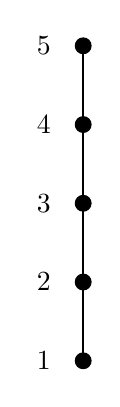
\begin{tikzpicture}
   \foreach \y in {1, 2, 3, 4, 5} {
    \node[circle,draw,fill=black,minimum size=2mm,inner sep=0pt,outer
    sep=0pt] at (0, \y - 1) {};
    \node at (-0.5, \y - 1) {$\clr{\y}$};
   }
   \foreach \y in {1, 2, 3, 4} {
    \draw[thick] (0, \y - 1) -- (0, \y);
   }
  \end{tikzpicture}
  \caption{Hasseho diagram uspořádáné množiny $(\clr{A}, \leq)$.}
  \label{fig:hasse-linear}
 \end{figure}
 Ve skutečnosti, Hasseho diagram \textbf{každého} lineárního uspořádání vypadá
 takto; liší se pouze počet prvků. Detaily si rozmyslíte za cvičení.
\end{example}

\begin{definition}[Dělitelnost]
 \label{def:delitelnost}
 Mějme čísla $m,n \in \N$. Říkáme, že $m$ \textbf{dělí} $n$, když existuje
 přirozené číslo $k \in \N$ takové, že $n = km$. Tento fakt zapisujeme jako $m
 \mid n$.
\end{definition}

\begin{example}[Uspořádání dělitelností]
 Relace $ \mid $ z \hyperref[def:delitelnost]{definice dělitelnosti} je ve
 skutečnosti uspořádání (důkaz jako cvičení), které \textbf{ale není lineární}.
 Jeho \hyperref[fig:hasse-delitelnost]{Hasseho diagram} na množině $\clr{A}
 \coloneqq \clr{[10]}$ je výrazně košatější.
 \begin{figure}[H]
  \centering
  \begin{tikzpicture}
   \node[circle,draw,fill=black,minimum size=2mm,inner sep=0pt,outer
   sep=0pt] (1) at (0, 0) {};
   \node[below=1mm of 1] {$\clr{1}$};

   \node[circle,draw,fill=black,minimum size=2mm,inner sep=0pt,outer
   sep=0pt] (2) at (-3, 1) {};
   \node[left=1mm of 2] {$\clr{2}$};

   \node[circle,draw,fill=black,minimum size=2mm,inner sep=0pt,outer
   sep=0pt] (3) at (-1, 1) {};
   \node[left=1mm of 3] {$\clr{3}$};

   \node[circle,draw,fill=black,minimum size=2mm,inner sep=0pt,outer
   sep=0pt] (5) at (1, 1) {};
   \node[right=1mm of 5] {$\clr{5}$};

   \node[circle,draw,fill=black,minimum size=2mm,inner sep=0pt,outer
   sep=0pt] (7) at (3, 1) {};
   \node[right=1mm of 7] {$\clr{7}$};

   \draw[thick] (1) -- (2);
   \draw[thick] (1) -- (3);
   \draw[thick] (1) -- (5);
   \draw[thick] (1) -- (7);

   \node[circle,draw,fill=black,minimum size=2mm,inner sep=0pt,outer
   sep=0pt] (4) at (-3, 2) {};
   \node[left=1mm of 4] {$\clr{4}$};

   \node[circle,draw,fill=black,minimum size=2mm,inner sep=0pt,outer
   sep=0pt] (8) at (-3, 3) {};
   \node[left=1mm of 8] {$\clr{8}$};

   \draw[thick] (2) -- (4);
   \draw[thick] (4) -- (8);

   \node[circle,draw,fill=black,minimum size=2mm,inner sep=0pt,outer
   sep=0pt] (8) at (-3, 3) {};
   \node[left=1mm of 8] {$\clr{8}$};

   \node[circle,draw,fill=black,minimum size=2mm,inner sep=0pt,outer
   sep=0pt] (6) at (-2, 2) {};
   \draw[thick] (2) -- (6);
   \draw[thick] (3) -- (6);
   \node[left=1mm of 6] {$\clr{6}$};

   \node[circle,draw,fill=black,minimum size=2mm,inner sep=0pt,outer
   sep=0pt] (9) at (-1, 2) {};
   \draw[thick] (3) -- (9);
   \node[right=1mm of 9] {$\clr{9}$};

   \node[circle,draw,fill=black,minimum size=2mm,inner sep=0pt,outer
   sep=0pt] (10) at (1, 2) {};
   \node[right=1mm of 10] {$\clr{10}$};
   \draw[thick] (2) -- (10);
   \draw[thick] (5) -- (10);
  \end{tikzpicture}
  \caption{Hasseho diagram uspořádané množiny $(\clr{A}, \mid)$.}
  \label{fig:hasse-delitelnost}
 \end{figure}
\end{example}

Lexikografické uspořádání je v principu uspořádání na slovech, ale může být
úspěšně použito třeba i pro uspořádání polynomů více proměnných. Funguje
následovně: slovem délky $n$ nazveme posloupnost $a_1a_2\ldots a_n$, kde $a_i$
je libovolné písmeno mezi \uv{a} a \uv{z}. Slovo $a_1a_2\ldots a_n$ je
lexikograficky níž než slovo $b_1b_2\ldots b_m$, pokud existuje $i \leq
\min(n,m)$ takové, že $a_1 = b_1 \wedge a_2 = b_2 \wedge \ldots \wedge a_{i-1} =
b_{i-1}$ a $b_i > a_i$.

Řečeno lidsky, o slově $a_1a_2\ldots a_n$ řeknu, že je níž než $b_1b_2\ldots
b_m$, když nějaké jeho písmeno $a_i$ je dřív v abecedě než písmeno $b_i$ na
stejném místě ve slově $b_1b_2\ldots b_m$. Pokud je jedno slovo plně součástí
druhého, lexikograficky níž je to kratší. Lexikografické uspořádání se obvykle
značí rovněž $ \leq $, ale pro přehlednost ho budeme značit třeba
$\leq_{\text{lex}}$.

\begin{example}[Lexikografické uspořádání]
 Jak si můžete ověřit (ale cvičení to nutně není), lexikografické uspořádání je
 lineární, takže jeho Hasseho diagram není dvakrát zajímavý. Pro úplnost zde
 ale přesto ukážeme \hyperref[fig:hasse-lex]{diagram} množiny
 \[
  \clr{A} \coloneqq \clr{\{a_1a_2 \mid a_i \in \{a,b,c\}\}},
 \]
 tedy množiny všech dvojpísmenných kombinací písmen \uv{a} až \uv{c}.
 \begin{figure}[H]
  \centering
  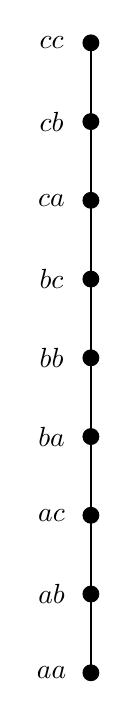
\begin{tikzpicture}
   \foreach \y in {1, 2, 3, 4, 5, 6, 7, 8, 9} {
    \node[circle,draw,fill=black,minimum size=2mm,inner sep=0pt,outer
    sep=0pt] at (0, \y - 1) {};
   }
   \foreach \y in {1, 2, 3, 4, 5, 6, 7, 8} {
    \draw[thick] (0, \y - 1) -- (0, \y);
   }
   \node at (-0.5, 0) {$\clr{aa}$};
   \node at (-0.5, 1) {$\clr{ab}$};
   \node at (-0.5, 2) {$\clr{ac}$};
   \node at (-0.5, 3) {$\clr{ba}$};
   \node at (-0.5, 4) {$\clr{bb}$};
   \node at (-0.5, 5) {$\clr{bc}$};
   \node at (-0.5, 6) {$\clr{ca}$};
   \node at (-0.5, 7) {$\clr{cb}$};
   \node at (-0.5, 8) {$\clr{cc}$};
  \end{tikzpicture}
  \caption{Hasseho diagram uspořádané množiny $(\clr{A}, \leq_{\text{lex}})$.}
  \label{fig:hasse-lex}
 \end{figure}
\end{example}

Velmi pěkné obrázky uspořádání vznikají i na množině všech množin $A$, tedy na
$2^{A}$, kde uspořádání je inkluzí $ \subseteq $. Tedy, nejníž je prázdná
množina, která leží uvnitř každé množiny, a nejvýš je množina $A$, ve které je
obsažena každá její podmnožina. Jeden malý příklad tu nakreslíme, určitě se vám
bude líbit.

\begin{example}
 Mějme množinu $A \coloneqq \{1,2,3\}$. Množinu $\clr{2^{A}}$ uspořádáme
 inkluzí, čili dvě podmnožiny $A$ jsou v relaci inkluze, když je jedna obsažena
 v druhé. Jeden příklad za všechny je třeba $\{1\} \subseteq \{1,3\}$.
 \hyperref[fig:hasse-power-set]{Hasseho diagram} takového uspořádání vidíte
 níže. V rámci úspory píšeme třeba $12$ místo množiny $\{1,2\}$.
 \begin{figure}[H]
  \centering
  \begin{tikzpicture}
   \node[circle,draw,fill=black,minimum size=2mm,inner sep=0pt,outer
   sep=0pt] (0) at (0, 0) {};
   \node[circle,draw,fill=black,minimum size=2mm,inner sep=0pt,outer
   sep=0pt] (1) at (-2, 2) {};
   \node[circle,draw,fill=black,minimum size=2mm,inner sep=0pt,outer
   sep=0pt] (2) at (0, 2) {};
   \node[circle,draw,fill=black,minimum size=2mm,inner sep=0pt,outer
   sep=0pt] (3) at (2, 2) {};
   \node[circle,draw,fill=black,minimum size=2mm,inner sep=0pt,outer
   sep=0pt] (12) at (-2, 4) {};
   \node[circle,draw,fill=black,minimum size=2mm,inner sep=0pt,outer
   sep=0pt] (13) at (0, 4) {};
   \node[circle,draw,fill=black,minimum size=2mm,inner sep=0pt,outer
   sep=0pt] (23) at (2, 4) {};
   \node[circle,draw,fill=black,minimum size=2mm,inner sep=0pt,outer
   sep=0pt] (123) at (0, 6) {};

   \draw[thick] (0) -- (1);
   \draw[thick] (0) -- (2);
   \draw[thick] (0) -- (3);
   \draw[thick] (1) -- (12);
   \draw[thick] (1) -- (13);
   \draw[thick] (2) -- (12);
   \draw[thick] (2) -- (23);
   \draw[thick] (3) -- (13);
   \draw[thick] (3) -- (23);
   \draw[thick] (12) -- (123);
   \draw[thick] (13) -- (123);
   \draw[thick] (23) -- (123);

   \node[below=1mm of 0]{$\clr{\emptyset}$};
   \node[left=1mm of 1]{$\clr{1}$};
   \node[left=1mm of 2]{$\clr{2}$};
   \node[right=1mm of 3]{$\clr{3}$};
   \node[left=1mm of 12]{$\clr{12}$};
   \node[left=1mm of 13]{$\clr{13}$};
   \node[right=1mm of 23]{$\clr{23}$};
   \node[above=1mm of 123]{$\clr{123}$};
  \end{tikzpicture}
  \caption{Hasseho diagram uspořádané množiny $(\clr{2^{A}}, \subseteq)$.}
  \label{fig:hasse-power-set}
 \end{figure}
\end{example}
Jako obvykle následuje několik cvičení na závěr sekce.

\begin{exercise}
 Udělejte cvičení rozmístěná po sekci. Konkrétně,
 \begin{enumerate}
  \item dokažte, že Hasseho diagram každého lineárního uspořádání má stejný tvar
   jako diagram na \hyperref[fig:hasse-linear]{obrázku~\ref*{fig:hasse-linear}}.
  \item dokažte, že relace dělitelnosti $ \mid $ je uspořádání na každé
   podmnožině přirozených čísel.
 \end{enumerate}
\end{exercise}

\begin{exercise}
 Explicitně popište všechny relace (na libovolné množině), které jsou zároveň
 ekvivalencí a (částečným) uspořádáním.
\end{exercise}

\begin{exercise}
 Řekněme, že $R$ a $S$ jsou uspořádání na množině $A$. Které z následujících
 relací jsou také uspořádáními na $A$?
  \begin{itemize}[itemsep=0pt]
  \item $R \cap S$ 
  \item $R \cup S$ 
  \item $R \setminus S$
  \item $R \circ S$
 \end{itemize}
\end{exercise}

\subsection{Matematická indukce}
\label{ssec:matematicka-indukce}

Indukce je základní důkazovou technikou v diskrétní matematice. Je to jeden
možný, ale zcela jistě nejoblíbenější, způsob, jak dokazovat libovolná tvrzení o
přirozených číslech, která jsou vlastně právě tím číselným oborem, který studuje
diskrétní matematika.

Princip indukce spočívá v tom, že přirozená čísla jsou definována v zásadě velmi
jednoduše. Libovolná množina, která má nějaký \uv{základní prvek} (třeba
jedničku) a spolu s každým prvkem má i jeho bezprostředního následníka (třeba to
číslo o jedna větší), je automaticky \uv{ta samá množina} jako přirozená čísla.

Pokud byste měli chuť se podívat na formální definici přirozených čísel a
dalších souvisejících věcí, doporučujeme vyhledat klíčová slova \emph{Peanova
aritmetika}, která je vlastně (možná kecám, ale myslím, že nejmenším možným)
systémem axiomů (kategoricky platných výroků), jenž buduje ryze logický základ
pro aritmetiku.

My si ale vystačíme s následujícím zjednodušením.

\begin{claim}[Definice přirozených čísel]
 Nechť $A$ je množina, která splňuje, že
 \begin{itemize}
  \item $1 \in A$,
  \item je-li $n \in A$, pak rovněž $n+1 \in A$.
 \end{itemize}
 Potom $A = \N$.
\end{claim}
\begin{proof}
 Nedokazuje se, je to axiom (konkrétně pátý) Peanovy aritmetiky.
\end{proof}

Žádáme, abyste si dali chvíli a zamysleli nad významem tvrzení. Zevrubně řečeno
říká, že, pokud umím dokázat, že
\begin{itemize}
 \item tvrzení platí pro první přirozené číslo a
 \item za předpokladu, že tvrzení platí pro $n$, platí pro $n + 1$,
\end{itemize}
pak dané tvrzení platí pro všechna přirozená čísla. Tyhle dva důkazy totiž
dohromady dávají následující (nekonečný) řetězec důkazů:
\begin{enumerate}
 \item (Nějaké) tvrzení platí pro $n = 1$.
 \item Jestliže tvrzení platí pro $n = 1$, pak platí pro $n = 2$.
 \item Jestliže tvrzení platí pro $n = 2$, pak platí pro $n = 3$.

 \centering $\vdots$
\end{enumerate}

Princip indukce asi není přehnaně složitý, ale získat dostatek zkušenosti, aby
jej člověk uměl neomylně aplikovat, je výrazně obtížnější. Pár příkladů snad s
tímto krokem pomůže. Budeme je záměrně formulovat jako lemmata či tvrzení,
jelikož indukce je v prvé řadě důkazová technika. Doporučujeme, abyste důkazy
četli se zvýšenou pozorností.

\begin{lemma}
 Pro každé $n \in \N$ platí
 \[
  \sum_{i=0}^{n} 2^{i} = 2^{n+1} - 1.
 \]
\end{lemma}
\begin{proof}
 Dokazujeme indukcí. Protože suma začíná od $0$, je prvním prvkem, pro který
 musí tvrzení platit, v tomto případě právě $n = 0$. Dosazením zjistíme, že
 \[
  \sum_{i=0}^{0} 2^{i} = 2^{0} = 1 = 2^{0 + 1} - 1
 \]
 tedy tvrzení platí pro $n = 0$. Předpokládáme, že tvrzení platí pro všech\-na
 přirozená čísla až do nějakého $n \in \N$ a z tohoto předpokladu odvodíme, že
 platí i pro $n + 1$. Počítáme
 \[
  \sum_{i=0}^{n + 1} 2^{i} = \sum_{i=0}^{n} 2^{i} + 2^{n+1}.
 \]
 Ovšem, z předpokladu dostaneme
 \[
  \sum_{i=0}^{n} 2^{i} = 2^{n+1}-1,
 \]
 což dohromady s předchozím výpočtem dává
 \[
  \sum_{i=0}^{n + 1} 2^{i} = \clr{\sum_{i=0}^{n} 2^{i}} + 2^{n+1} = \clr{2^{n +
  1} - 1} + 2^{n+1} = 2 \cdot 2^{n+1} - 1 = 2^{n+2} - 1,
 \]
 jak jsme chtěli ukázat. Důkaz je podle principu indukce ukončen.
\end{proof}

\begin{lemma}
 \label{lemma:deleni-trojkou}
 Pro všechna $n \in \N$ platí, že
 \[
  3 \mid n \Rightarrow 3 \mid n^2,
 \]
 tedy, pokud $3$ dělí $n$, pak $3$ dělí $n^2$.
\end{lemma}
Tady by se jistě leckdo rád odvolal třeba na prvočíselné rozklady. Je ale dobré
si uvědomit, že fakt, že každé přirozené číslo má jednoznačný rozklad na
prvočísla, není samozřejmý. Ve skutečnosti zabere určitou práci toto dokázat. Či
vy jste viděli nějaký přímočarý důkaz, že jdou čísla rozkládat na prvočísla?
Opravdu lze \emph{každé} číslo rozložit na prvočísla a opravdu to lze
\emph{pouze jediným způsobem}?

\begin{enhproof}[lemmatu~\ref{lemma:deleni-trojkou}]
 Dokazujeme indukcí.

 První přirozené číslo, pro které má smysl tvrzení dokázat, je $n = 3$. Pak
 vskutku $3 \mid n = 3$ a $3 \mid n^2 = 9$.

 Předpokládejme, že výrok $3 \mid n \Rightarrow 3 \mid n^2$ platí pro nějaké
 $n \in \N$. Nejbližší další přirozené číslo po $n$, které je dělitelné $3$, je
 $n + 3$. Tedy, víme, že když $3 \mid n$, pak $3 \mid n + 3$ a také $3 \mid
 n^2$. Z těchto dvou faktů odvodíme, že $3 \mid (n+3)^2$.

 Máme $(n + 3)^2 = n^2 + 6n + 9$. Protože $3 \mid 6$ a $3 \mid 9$, také $3 \mid
 6n + 9$. Předpokládáme, že $3 \mid n^2$, dohromady tudíž $3 \mid n^2 + 6n + 9 =
 (n+3)^2$, jak jsme chtěli.
\end{enhproof}

Tři cvičení nakonec.
\newpage
\begin{exercise}
 Dokažte indukcí, že
 \[
  \sum_{i=1}^{n} i 2^{i} = (n - 1)2^{n+1} + 2.
 \]
\end{exercise}

\begin{exercise}[Fibonacciho čísla a zlatý řez]
 Tak zvaná \emph{Fibonacciho} posloupnost je definována tak, že další člen
 dostanu jako součet dvou předchozích. Formálně, $F_0 = 0, F_1 = 1$ a $F_n =
 F_{n - 1} + F_{n - 2}$, kde $n \in \N$. Dokažte indukcí, že
 \[
  F_n \leq \left( \frac{1+\sqrt{5}}{2} \right) ^{n-1}
 \]
 pro všechna $n \geq 0$.

 Číslu  $(1+\sqrt{5}) / 2$ se někdy říká hodnota \uv{zlatého řezu} (protože je
 to v jistém smyslu \emph{ideální} poměr mezi délkami dvěma bezprostředních
 úseček -- internet poví víc). Jestli si někdy ukážeme limity, pak dokážeme
 tento výsledek zdokonalit v tom smyslu, že platí
 \[
  \frac{F_n}{F_{n-1}} \xrightarrow{n \to \infty} \frac{1+\sqrt{5}}{2}. 
 \]
\end{exercise}

\begin{exercise}
 Nakresleme $n$ přímek v rovině, a to tak, že
 \begin{itemize}
  \item žádné 2 nejsou rovnoběžné a
  \item žádné 3 se neprotínají v jednom bodě.
 \end{itemize}
 Dokažte indukcí, že takhle nakreslené přímky rozdělují rovinu na $n(n+1) / 2 +
 1$ částí.
\end{exercise}

